\documentclass[a4paper]{scrartcl}

\usepackage[english]{babel}

\usepackage{amsmath, amssymb, amsfonts, amsthm, mathtools}
\usepackage{graphicx}
\usepackage{xcolor}

\usepackage{csquotes}

\usepackage{biblatex}
\bibliography{refs}

\definecolor{GoetheBlue}{rgb}{0,0.38,0.56}
\usepackage[%
  colorlinks = true,
  citecolor  = GoetheBlue,
  linkcolor  = GoetheBlue,
  urlcolor   = GoetheBlue,
  unicode,
]{hyperref}


% Credits to `https://tex.stackexchange.com/questions/348651/c-code-to-add-in-the-document`
\definecolor{mGreen}{rgb}{0,0.6,0}
\definecolor{mGray}{rgb}{0.5,0.5,0.5}
\definecolor{mPurple}{rgb}{0.58,0,0.82}
\definecolor{backgroundColour}{rgb}{0.95,0.95,0.92}

\usepackage{listings}
\lstdefinestyle{CStyle}{
    backgroundcolor=\color{backgroundColour},   
    commentstyle=\color{mGreen},
    keywordstyle=\color{magenta},
    numberstyle=\tiny\color{mGray},
    stringstyle=\color{mPurple},
    basicstyle=\footnotesize,
    breakatwhitespace=false,         
    breaklines=true,                 
    captionpos=b,                    
    keepspaces=true,                 
    numbers=left,                    
    numbersep=5pt,                  
    showspaces=false,                
    showstringspaces=false,
    showtabs=false,                  
    tabsize=2,
    language=C,
    keywords={
        uint32_t, uint64_t, return, struct, define, unsigned, int
    }
}

\usepackage[vlined,ruled,linesnumbered]{algorithm2e}
\DontPrintSemicolon
\SetKwFunction{RNG}{rng()}
\SetKwFunction{FLIP}{flip()}


\setkomafont{sectioning}{\normalfont\scshape}


\title{Random Number Generation in the Pim-Architecture}
\subtitle{Research Project Report}
\author{Lukas Geis}
\date{}

\begin{document}
\maketitle
\tableofcontents

\newpage
\section{Introduction} \label{sec:1}
A \emph{Pseudo}-\textsc{RandomNumberGenerator} (\textsc{Rng}) is the basis of all random functionality in practice.
We can generate a series of (\emph{pseudo}) random numbers to simulate \emph{true} randomness to a certain degree.
This way, we can create random models to create diverse data sets or approximate complex problems efficiently.

The \textsc{Upmem-Pim}\footnote{\url{https://www.upmem.com/}} architecture is the first publicly-available real-world processing-in-memory (\textsc{Pim}) architecture.
It combines traditional DRAM memory arrays with general-purpose in-order cores, called DRAM Processing Units (DPUs), integrated in the same chip.

This report describes the implementation and benchmarks of a handful of widely-used \textsc{Rng}'s as well as several algorithms for uniformly sampling integers in a given range (\textsc{Sampler}) in the \textsc{Upmem-Pim} toolchain using the C programming language.
The code can be found \href{https://github.com/lukasgeis/upmem-rng}{here}\footnote{\url{https://github.com/lukasgeis/upmem-rng}}.
\hyperref[sec:2]{Section 2} provides algorithm details of the implemented \textsc{Rng}'s.
\hyperref[sec:3]{Section 3} provides algorithm details of the implemented \textsc{Sampler}'s.
\hyperref[sec:4]{Section 4} benchmarks the implementations and analyzes the results.


\section{Random Number Generators} \label{sec:2}
In this section, we provide a short overview of the implemented \textsc{Rng}'s.
In total, $6$ different \textsc{Rng}'s were implemented and benchmarked.
As the \textsc{Upmem-Pim} only has efficient support for $32$-bit numbers, every \textsc{Rng} were implemented in its $32$-bit variant.
A short overview of the comparison of all \textsc{Rng}'s except the \hyperref[sec:2.3]{Subtract-With-Carry} \textsc{Rng} can be seen \href{https://www.pcg-random.org/}{here}\footnote{\url{https://www.pcg-random.org/}}.

\subsection{XorShift} \label{sec:2.1}
The first and most trivial \textsc{Rng} implemented was the XorShift (XS) \textsc{Rng}~\cite*{XS}.
In spirit of its name, it only consists of three BitShifts followed by a Xor:
\begin{lstlisting}[style=CStyle]
uint32_t gen_xs32(struct xs32 *rng) {
    uint32_t x = rng->x;
    x ^= x << 13;
    x ^= x >> 17;
    x ^= x << 5;
    return rng->x = x;
}
\end{lstlisting}
While its simplicity makes it very predictable, it should also be the fastest one as it only incorporates bit operations which all can be efficiently executed on the DPU.


\subsection{MersenneTwister} \label{sec:2.2}
The second \textsc{Rng} implemented is the MersenneTwister (MS) \textsc{Rng}~\cite*{MT}.
The key idea is to define a series $x_i$ through a simple recurrence relation, and then output numbers of the form $x_i^T$ where $T$ is an invertible $\mathbb{F}_2$-matrix called a tempering matrix.\footnote{\url{https://en.wikipedia.org/wiki/Mersenne_Twister}}.
While the complete \textsc{Rng} is too complex to put here\footnote{See the full code here: \url{https://github.com/lukasgeis/upmem-rng/blob/main/includes/rng.c}}, we will provide a quick overwie over its parameters:
\begin{lstlisting}[style=CStyle]
#define MT_N 624            // Parameter `N`
#define MT_M 397            // Parameter `M`
#define MT_A 0x9908b0dfU    // Constant Vector `A`
#define MT_U 0x80000000U    // Mask for most significant `W - R` Bits
#define MT_L 0x7fffffffU    // Mask for least significant `R` Bits

struct mt32 {
    uint32_t mt[MT_N];
    int mti;
};
\end{lstlisting}
As seen in line $8$, the \textsc{Rng} needs at least a working area of $624$ words, making it quite large in comparison to other \textsc{Rng}'s.
This leads to the requirement of using the compiler-flag 
\begin{center}
    -DSTACK\_SIZE\_DEFAULT=2800
\end{center}
in the \texttt{dpu-upmem-dpurte-clang} compiler used to compile the DPU source code.


\subsection{SubtractWithCarry} \label{sec:2.3}
The third \textsc{Rng} implemented is the SubtractWithCarry (SC) \textsc{Rng}~\cite*{SC}.
This \textsc{Rng} is defined by the following recurrence relation:
\begin{align*}
    x(i) &= (x(i - S) - x(i - R) - cy(i - 1)) \mod M \\
    \text{ where }\,\, cy(i) &= \left\{\begin{array}{cl}
        1, & \text{ if $x(i - S) - x(i - R) - cy(i - 1) < 0$} \\
        0, & \text{ otherwise }
    \end{array}\right.
\end{align*}
with $0 < S < R$ and $M = 2^W$ where $W$ is the word size.
In our case, we used $S = 8, R = 20, M = 2^{32}$.
\vspace*{\fill}
\\
The last three \textsc{Rng}'s act as a form of a baseline since they are all \textsc{Rng}'s that are either complex or very efficient if we have access to fast multiplication which is not the case in the \textsc{Upmem-Pim} architecture.
\\ \\ 

\newpage
\subsection{Lehmer} \label{sec:2.4}
The fourth \textsc{Rng} implemented is the Lehmer (LM) \textsc{Rng}~\cite*{LM}.
The general formula is 
\begin{align*}
    X_{k + 1} = \alpha \cdot X_k \mod m
\end{align*}
where the modulus $m$ is a prime number or power of a prime number, the multiplier $\alpha$ is an element of high multiplicative order modulo $m$.
We used the MINSTD parameters of $m = 2^{31} - 1 = 2147483647$ and $\alpha = 7^5 = 16807$~\cite*{MINSTD}.


\subsection{PCG} \label{sec:2.5}
The fifth \textsc{Rng} implemented was the PCG32 (PCG) \textsc{Rng}~\cite*{PCG}.
While we generate $32$-bit numbers, the state consists of two $64$-bit numbers:
\begin{lstlisting}[style=CStyle]
struct pcg32 {      
    uint64_t state; // RNG state.  All values are possible.
    uint64_t inc;   // Always odd. Controls which RNG sequence is selected
};
\end{lstlisting}
While the generation of the next state is short, it not only uses $64$-bit numbers but also multiplication of two $64$-bit numbers which is very inefficient on the DPU:
\begin{lstlisting}[style=CStyle]
uint32_t gen_pcg32(struct pcg32 *rng) {
    uint64_t oldstate = rng->state;
    rng->state = oldstate * 6364136223846793005ULL + rng->inc;
    uint32_t xorshifted = ((oldstate >> 18u) ^ oldstate) >> 27u;
    uint32_t rot = oldstate >> 59u;
    return (xorshifted >> rot) | (xorshifted << ((-rot) & 31));
} 
\end{lstlisting}

\subsection{ChaCha} \label{sec:2.6}
The last \textsc{Rng} implemented is the ChaCha (CHA) \textsc{Rng}~\cite*{CHA} which is a variation of the Salsa20\footnote{\url{https://en.wikipedia.org/wiki/Salsa20}} \textsc{Rng}.
Its internal state consists of a $4x4$-Matrix of $32$-bit words and also has a buffer of the same size.
The last $4$ words of the states simulate a $128$-bit counter and are incremented in each iteration.
The main part of the algorithm consists of the following schema:
\begin{lstlisting}[style=CStyle]
#define CHACHA_ROTL32(x, n) (((x) << (n)) | ((x) >> (32 - (n))))

#define CHACHA_QUARTERROUND(x, a, b, c, d) \
    x[a] = x[a] + x[b]; x[d] ^= x[a]; x[d] = CHACHA_ROTL32(x[d], 16); \
    x[c] = x[c] + x[d]; x[b] ^= x[c]; x[b] = CHACHA_ROTL32(x[b], 12); \
    x[a] = x[a] + x[b]; x[d] ^= x[a]; x[d] = CHACHA_ROTL32(x[d],  8); \
    x[c] = x[c] + x[d]; x[b] ^= x[c]; x[b] = CHACHA_ROTL32(x[b],  7)

#define ROUNDS 20
\end{lstlisting}
\newpage
\noindent and the following round-system:
\begin{lstlisting}[style=CStyle]
for (unsigned int i = 0; i < ROUNDS; i += 2) {
    // Column Round
    CHACHA_QUARTERROUND(rng->buffer, 0, 4,  8, 12);
    CHACHA_QUARTERROUND(rng->buffer, 1, 5,  9, 13);
    CHACHA_QUARTERROUND(rng->buffer, 2, 6, 10, 14);
    CHACHA_QUARTERROUND(rng->buffer, 3, 7, 11, 15);
    // Diagonal Round
    CHACHA_QUARTERROUND(rng->buffer, 0, 5, 10, 15);
    CHACHA_QUARTERROUND(rng->buffer, 1, 6, 11, 12);
    CHACHA_QUARTERROUND(rng->buffer, 2, 7,  8, 13);
    CHACHA_QUARTERROUND(rng->buffer, 3, 4,  9, 14);
}
\end{lstlisting}





\section{Uniform Integer Sampling} \label{sec:3}
We now can sample random unsigned integers with $32$-bits.
This alone, however, is often useless as we might only need to generate a random number between $1$ and $10$ for example.
Hence, we somehow need to convert our random number in the interval $[0,2^{32})$ uniformly to a number in the interval $[0,s)$ for some $s \in \mathbb{N}$.
Since simple solutions like the classic C-line:
\begin{center}
    \texttt{rand() \% s}
\end{center}
lack uniformity, we need a better approach. 
For simplicity, we assume we can generate a \emph{uniform} random number in the interval $[0,2^L)$ for $L = 32$ using the function \texttt{rng()}.
Furthermore, we assume $s$ is given as a parameter for every following algorithm.
\\
\\
Finally, we will skip extensive explanations of the following \textsc{Sampler}'s.
For the first three, please refer to~\cite*{Lemire} for better explanations.


\subsection{OpenBSD} \label{sec:3.1}
The OpenBSD \textsc{Sampler} is an algorithm used in the $C$ standard library in OpenBSD and macOS.
The Go language also has adopted this algorithm with minor implementation differences.
The algorithm is given by the following pseudocode: 
\begin{algorithm}
    \caption{OpenBSD}
    $t \leftarrow (2^L - s) \mod s$\;
    $x \leftarrow$ \RNG\;
    \While{$x < t$}{
        $x \leftarrow$ \RNG\;
    }
    \KwRet{$x \mod s$}\;
\end{algorithm}
\\
The key idea is to apply simple rejection sampling to ensure uniformity.
This algorithm uses $2$ division operations which are not very efficient on the DPU.


\subsection{Java} \label{sec:3.2}
The Java \textsc{Sampler} is an algorithm used in the Java \texttt{Random class} and aims to only use one division operation in expectation.
The algorithm is given by the following pseudocode: 
\begin{algorithm}
    \caption{Java}
    $x \leftarrow$ \RNG\;
    $r \leftarrow x \mod s$\;
    \While{$x - r > 2^L - s$}{
        $x \leftarrow$ \RNG\;
        $r \leftarrow x \mod s$\;
    }
    \KwRet{$r$}\;
\end{algorithm}
\\
While in theory, we could have an unbounded number of division operations, in expectation, we only have $\frac{1}{p}$ for $p = 1 - \frac{2^L \mod s}{2^L} \geq \frac{1}{2}$ and hence for small $s$ no more than one division operation in expectation.


\subsection{Lemire} \label{sec:3.3}
Lemire's \textsc{Sampler} aims to completely minimize the number of costly division operations by reducing the number of expected divisions to $\frac{s}{2^L}$ and capping the number of division operations at $1$, meaning that for small $s$, we have no divison operation.
The algorithm is given by the following pseudocode: 
\begin{algorithm}
    \caption{Lemire}
    $x \leftarrow$ \RNG\;
    $m \leftarrow x \times s$\;
    $l \leftarrow m \mod 2^L$\;
    \If{$l < s$}{
        $t \leftarrow (2^L - s) \mod s$\;
        \While{$l < t$}{
            $x \leftarrow$ \RNG\;
            $m \leftarrow x \times s$\;
            $l \leftarrow m \mod 2^L$\;
        }
    }
    \KwRet{$m \div 2^L$}\;
\end{algorithm}
\\
Here, operations {\small mod $2^L$} and {\small $\div\,2^L$} can be implemented using a simple Bit-And and Bit-Shift.
While we minimize division operations, we also introduce a multiplication operation of two $64$-bit numbers in line $3$ which is very costly on a DPU.



\subsection{Flips} \label{sec:3.4}
The Flips \textsc{Sampler} uses a different approach by building up the final number bit-by-bit and resetting some of its progress if we exceed the threshold $s$~\cite*{Flips}.
Let \texttt{flip()} be a function that returns a single uniform random bit (can be implemented by \texttt{rng() \& 1}).
The algorithm is given by the following pseudocode: 
\begin{algorithm}
    \caption{Flips}
    $v \leftarrow 1$\;
    $d \leftarrow 0$\;
    \While{\emph{true}}{
        $d = 2 \cdot d\,+$ \FLIP\;
        $v = 2 \cdot v$\;
        \If{$v \geq s$}{
            \If{$d < s$}{
                \KwRet{$d$}\;
            }
            $v \leftarrow v - s$\;
            $d \leftarrow d - s$\;
        }
    }
\end{algorithm}
\\
Note that we can only draw $32$ bits at a time, we store the unused $31$ in a buffer and use them up until we draw a new random number.


\subsection{RoundReject (Variations)} \label{sec:3.5}
The main idea of the RoundReject (RR) \textsc{Sampler} is to only look at the bits of the random number that are relevant to $s$, namely the last $\lfloor\log_2(s)\rfloor + 1$ bits - and then use rejection sampling to generate a random number in the interval $[0,s)$.
The algorithm is given by the following pseudocode: 
\begin{algorithm}
    \caption{RoundReject}
    \tcc{Number of leading zeros in the binary representation of $s$}
    $l \leftarrow$ \texttt{$s$.leading\_zeros()}\;
    $m \leftarrow (1 << (32 - m)) - 1$\;
    $x \leftarrow$ \RNG \& $m$\;
    \While{$x \geq s$}{
        $x \leftarrow$ \RNG \& $m$\;
    }
    \KwRet{$x$}\;
\end{algorithm}
\\
\texttt{$s$.leading\_zeros()} can be achieved using the compiler-builtin function \texttt{\_\_builtin\_clz($s$)}.
\\
Since for small $s$, it might be wasteful to generate a new random number in each iteration and hence throw the $31 - \lfloor\log_2(s)\rfloor$ away, we create the following variations of the RR \textsc{Sampler}.

\paragraph*{RoundRejectBuffered (RRB)} 
Simply store all bits generated by \texttt{rng()} and use them in the next round instead of drawing a new random number every time.
If the remaining unused bits are not enough to fill up the required bits, draw a new number an concatenate the required bits.

\paragraph*{RoundRejectFlips (RRF)}
This is a combination of the RR and the Flips \textsc{Sampler}.
Since the longest part of Flips for bigger $s$ is building up the first batch of required bits, we skip that step by substituting the \glqq first round\grqq{} of Flips by one round of RR and then proceed with the original Flips algorithm.





\section{Benchmarks} \label{sec:4}
In this section, we discuss the most important benchmarks for these implementations.
The benchmark-code can also be found in the same GitHub-repository.
Note that we ran each benchmark only on 1 DPU at a time, since every experiment indicated that there was no time loss if multiple DPUs were running at the same time (except for the initial load-overhead which was not part of the benchmark hence excluded).
Thus, every result can be achieved on all DPUs at the same time (which in our case are about $2500$).
Every DPU has a capacity to have up to $22$ tasklets run parallel at the same time - hence every result in this section will be presented as a function of number of tasklets.

\subsection{Rng Benchmarks}
In this section, we will shortly review the execution time of each \textsc{Rng} on the DPU as well as on the CPU in comparison.
The results on the DPU can be seen in \hyperref[fig:1]{Figure 1}.
Clearly, XS yields the best results, needing less than $3$ seconds in total for $N = 10^7$ generated random numbers.
There is a slight increase in execution time starting from $11$ tasklets up to the end, but it stays under $4$ seconds nonetheless.
The next best \textsc{Rng} is SC, followed by MT, then CHA, LM, and finally PCG, which needs more than $40$ seconds at $1$ tasklet and more than $80$ seconds at $22$ tasklets.
This translates to our hypothesis, that \textsc{Rng}'s like XS, SC, and MT are better on the DPU because they do not require costly multiplications or $64$-bit numbers.
Every \textsc{Rng} seems to achieve a constant time regardless of number of tasklets up to $11$ tasklets before taking on linear growth in exeuction time.
This trend however is better observed in the right graphic which depicts the total number of bytes generated per second by all tasklets combined for each \textsc{Rng}.
The number is given by the conversion \[
    \underbrace{4}_{\text{Bytes in \texttt{uint32\_t}}} \cdot \underbrace{10^7}_{N} \cdot \underbrace{n_T}_{\text{Number of Tasklets}} / \underbrace{t_T}_{\text{Execution time in seconds}}
\] 
Here, we can clearly see that for more than $11$ tasklets, there is neither an additional benefit nor an additional cost for using more tasklets.
Using XorShift, we can achieve up to roughly $200$MB generated per second which translates to about $500$GB per second when using all $2500$ DPU modules.
\\

\begin{figure}[!htb] \label{fig:1}
    \makebox[\textwidth][c]{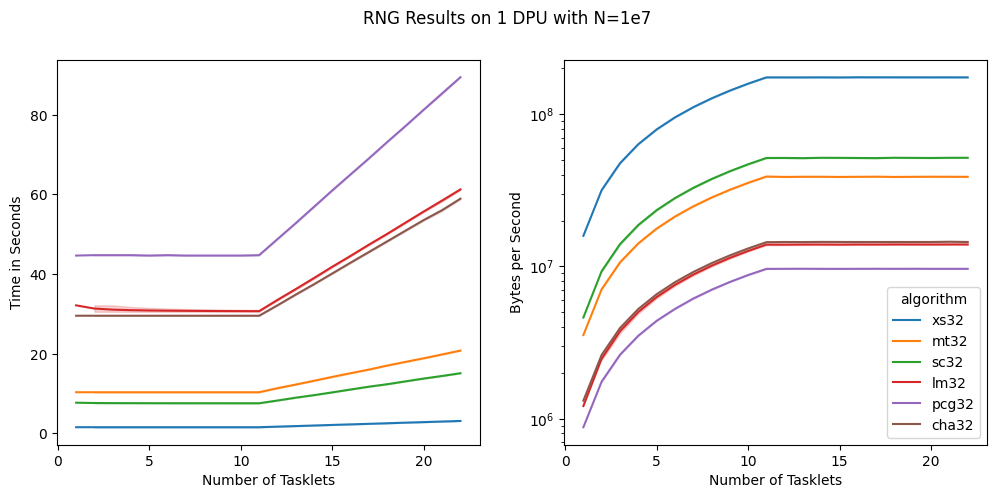
\includegraphics[width=1.15\textwidth]{img/dpu_rng.png}}
    \caption{
        Measured time and generated bytes per second taken by one DPU for generating $N = 10^7$ numbers with the respective \textsc{Rng}'s as a function of number of tasklets.        
    }    
\end{figure}

\begin{figure}[!htb] \label{fig:2}
    \makebox[\textwidth][c]{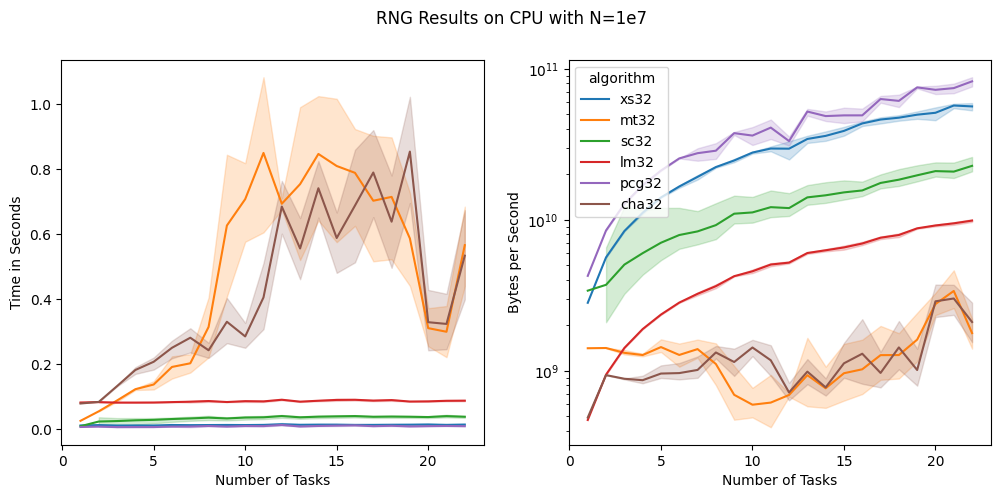
\includegraphics[width=1.15\textwidth]{img/cpu_rng.png}}
    \caption{
        Measured time and generated bytes per second taken by CPU for generating $N = 10^7$ numbers with the respective \textsc{Rng}'s as a function of number of tasks.        
    }    
\end{figure}

\clearpage
In comparison, we can see the results on the CPU in \hyperref[fig:2]{Figure 2}.
We will not go into too much detail about these results as they are only meant for a comparison with the DPU results - which are the main focus of this project.
We can clearly see that PCG and XorShift are the fastest \textsc{Rng}'s which is plausible considering the complexity of their generation code.
While MT was the third fastest \textsc{Rng} on the DPU, it is the slowest among the \textsc{Rng}'s on the CPU.
SC is still better than LM, MT and CHA, only beaten by the previously worse PCG.


\subsection{Sampler Benchmarks}
In this section, we will shortly review the execution time (and bytes generated per second) of each \textsc{Sampler} on the DPU as well as on the CPu in comparison.
We generated a random integer in the interval $[0,s)$ for every $2 \leq s \leq 10^9$ for every \textsc{Sampler} and added up the total computation time.
We also did this experiment one time using the XorShift-\textsc{Rng} - the fastest \textsc{Rng} on the DPU - and the PCG-\textsc{Rng} - the slowest \textsc{Rng} on the DPU - to account for the impact of the running time of generating a random number.
\\
\\
We can see the results on the DPU using the XS-\textsc{Rng} in \hyperref[fig:3]{Figure 3}.
The fastest \textsc{Sampler} is RR, closely followed by RRF and RRB, then by Java, OpenBSD, Lemire, and finally Flips.
This was to be expected since RR and its variants only use cheap and efficient operations like masking, addition and comparisons - with the exception of the one-time-use of \texttt{\_\_builtin\_clz()}.
Java and OpenBSD are also quite fast since they have a bounded number (or expected bounded) of costly division operations but no further inefficient operations.
While Lemire minimizes the number of divisions, it has a very costly multiplication operation of two $64$-bit integers which can happen several times.
Flips being last place also was to be expected since for bigger $s$, we will have to take $\log_2(s)$ steps to reach the first point where we can accept or reject a generated integer.
\\
On the right, we can see that RR achieves a throughput of roughly $70$MB generated per second while Flips only achieves a throughput of about $6$MB generated per second.
We can also see the same phenomenon we saw earlier: there is neither an additional benefit nor an additional cost for using more tasklets.
\\
\\
In comparion, if we use the PCG-\textsc{Rng} instead (\hyperref[fig:4]{Figure 4}), the results now differ at the top.
While Flips, and then Lemire, is still the slowest \textsc{Sampler}, the fastest one is now RRF, followed by Java, then OpenBSD and finally RR and RRF.
This makes sense since RRF minimizes the number of uses of \textsc{rng()} while RR enables rejecting many unused bits for smaller $s$ in comparison.
Here we achieve a maximal throughput of roughly $8$MB generated per second using RRF and about $4$MB generated per second using Flips.
Hence, when using a worse \textsc{Rng}, the difference between the best and the worst \textsc{Sampler} narrows.
\\


\begin{figure}[!htb] \label{fig:3}
    \makebox[\textwidth][c]{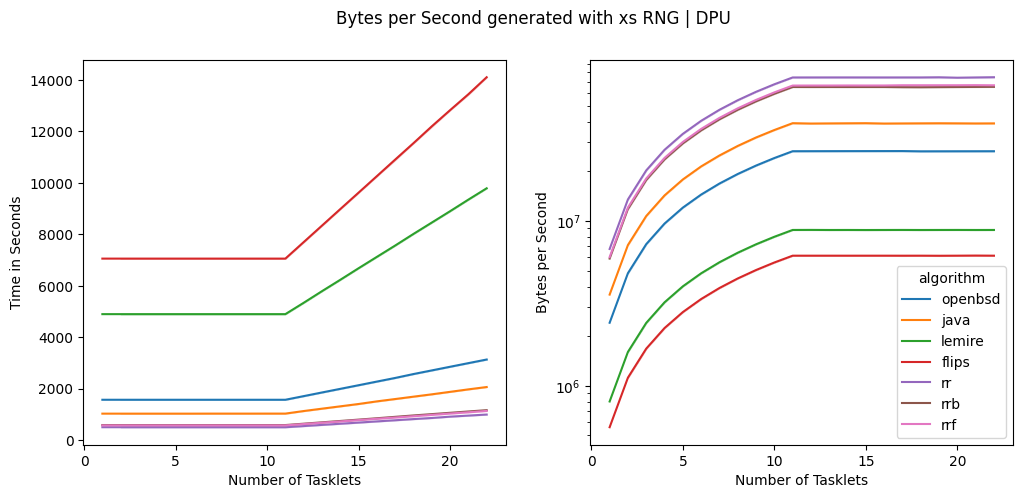
\includegraphics[width=1.15\textwidth]{img/dpu_sampling_xs.png}}
    \caption{
        Measured time and generated bytes per second taken by one DPU for generating numbers in range $[0,s)$ for all $s = 2..10^9$ with the respective \textsc{Sampler}'s as a function of number of tasklets. \textsc{Rng} used was XS.        
    }    
\end{figure}


\begin{figure}[!htb] \label{fig:4}
    \makebox[\textwidth][c]{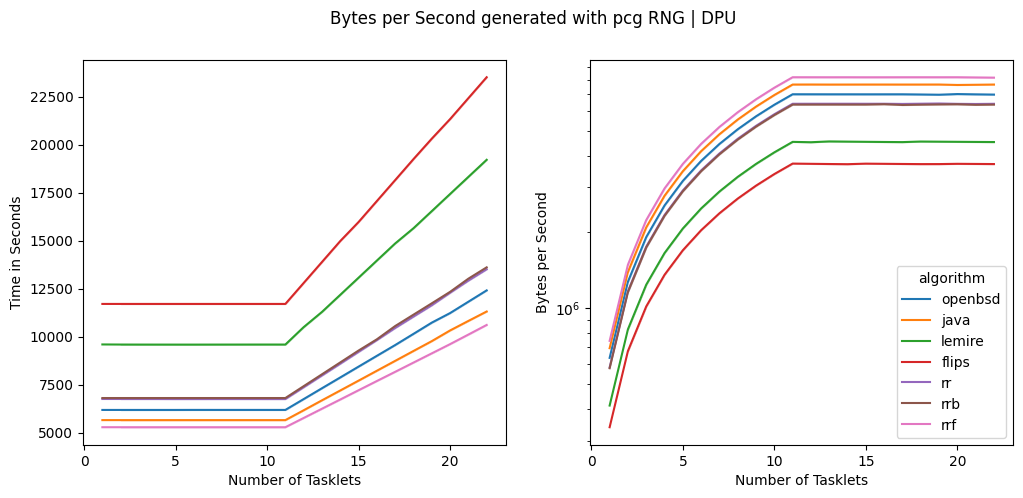
\includegraphics[width=1.15\textwidth]{img/dpu_sampling_pcg.png}}
    \caption{
        Measured time and generated bytes per second taken by CPU for generating numbers in range $[0,s)$ for all $s = 2..10^9$ with the respective \textsc{Sampler}'s as a function of number of tasks. \textsc{Rng} used was XS.        
    }   
\end{figure}


\begin{figure}[!htb] \label{fig:5}
    \makebox[\textwidth][c]{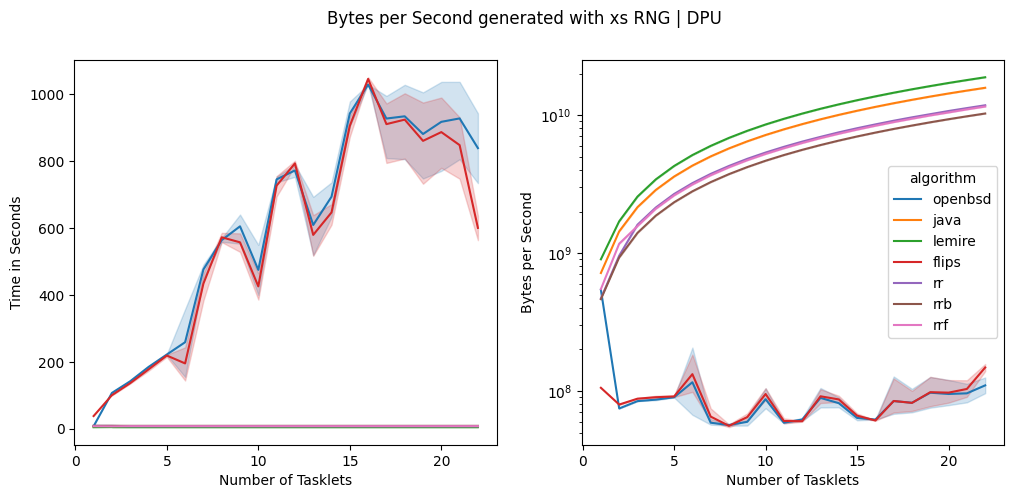
\includegraphics[width=1.15\textwidth]{img/cpu_sampling_xs.png}}
    \caption{
        Measured time and generated bytes per second taken by one DPU for generating numbers in range $[0,s)$ for all $s = 2..10^9$ with the respective \textsc{Sampler}'s as a function of number of tasklets. \textsc{Rng} used was PCG.      
    }   
\end{figure}


\begin{figure}[!htb] \label{fig:6}
    \makebox[\textwidth][c]{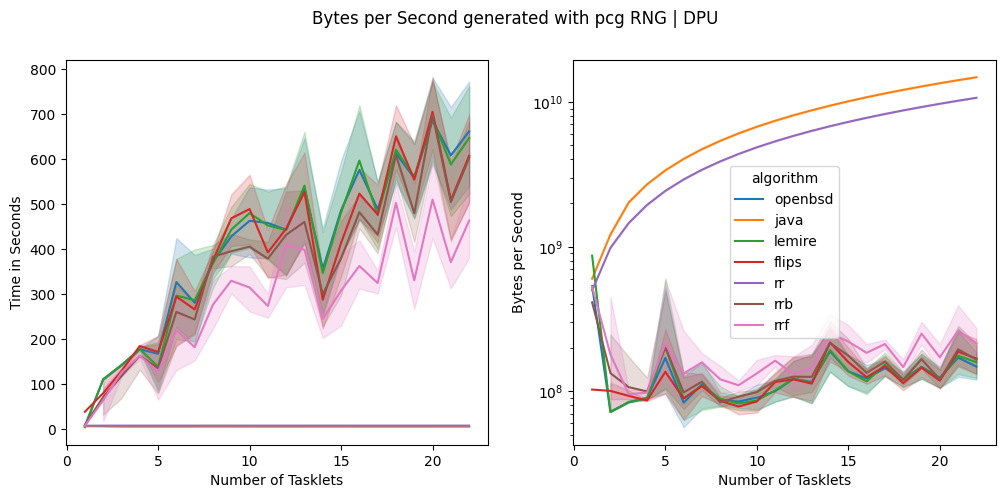
\includegraphics[width=1.15\textwidth]{img/cpu_sampling_pcg.png}}
    \caption{
        Measured time and generated bytes per second taken by CPU for generating numbers in range $[0,s)$ for all $s = 2..10^9$ with the respective \textsc{Sampler}'s as a function of number of tasks. \textsc{Rng} used was PCG.    
    }   
\end{figure}

\clearpage
If we look at the results of the same experiment on the CPU in comparison (\hyperref[fig:5]{Figure 5} and \hyperref[fig:6]{Figure 6}), we can clearly see that almost all \textsc{Sampler} - with the exception of Flips and OpenBSD - achieve an execution time of under $10$ seconds when using the XS-\textsc{Rng}.
Here, Lemire performs the best, followed by Java, RR, RRF, and RRB.
When using the PCG-\textsc{Rng}, only Java and RR perform quite well while the rest is way worse (and shaky). 
This might be due to some external issues (like Power-Management, etc.), but it was not studied and should be ignore instead as it is of no significant importance in this research project.

\printbibliography


\end{document}

